\documentclass[A4,twoside]{ctexart}
%\usepackage{slashbox}\backslashbox
\usepackage{aappss}
%\renewcommand\baselinestretch{1.235}\protect
\renewcommand\baselinestretch{2.0}\protect
\abovedisplayshortskip 0 pt plus 3pt
\belowdisplayshortskip 6 pt plus 2pt minus 2pt
\abovedisplayskip 6 pt plus 2pt minus 2pt
\belowdisplayskip 6 pt plus 2pt minus 2pt
% \info{2015}{64}{1}{01{}} \infodate{2015.0.0.}{2015.0.0.}
%=================== Text begin here ==============================

% 正文开始

\begin{document}\apsname

\title{非完整力学与控制\fivestar}

\author{王定文$^{1)\dag}$ \quad 高普云$^{1)}$}
\address{1)}{国防科技大学, 航天科学与工程学院, 长沙 \quad 410072}

\abstract{非完整约束的不可积性是非完整力学的困难所在。而非完整约束的来源是非完整力学研究中常被忽视的问题。本文从非完整约束的物理背景出发,揭示出非完整力学的控制本质。从控制的观点可以统一非完整系统的不同模型(如Chetaev模型和Vacco模型)。我们指出非完整力学仍然处于分析力学的理论框架内,不同模型的区别仅在于它们各自暗含的控制力不同。}

\keywords{非完整力学,控制论,Chetaev模型,Vacco模型}

\pacs{45.05.+x,45.20.Jj,45.80.+r}

\cmail{wangdingwen0618@gmail.com \quad 电话: 15116442661}


\section{引言}
\label{sec:intr}
非完整力学作为分析力学的一个分枝,其研究对象是一类特殊的力学系统,即含非完整约束的系统。一般所说的非完整约束有如下形式:
\begin{equation}
  \label{eq:nhcon}
  f_{\alpha}(\dot{q}_1,\dot{q}_2,\ldots,\dot{q}_n;q_1,q_2,\ldots,q_n;t)=0,\quad(\alpha=1,\ldots,m)
\end{equation}
其中$q$是广义坐标,$n$是广义坐标的数目,$m$是非完整约束的数目。

在Lagrange发展分析力学时并没有非完整约束的概念,在他那里所谓约束就是指对系统坐标的限制。直到1894年,Hertz把如\eqref{eq:nhcon}这样的约束命名为非完整约束,从此诞生了非完整力学\supercite{1}。简单来说,非完整约束的特点是约束方程中包含坐标的导数而且导数项不能通过积分的手段消去。

分析力学中的约束会导致系统自由度数减少,使得很多不能或难于用Newton力学处理的问题得到解决,而且由分析力学方法得到的动力学方程具有与坐标无关的形式不变性,其意义也早已超出力学范围。但在非完整力学中,非完整约束的引入却往往使问题更加复杂。比如虚位移这个在分析力学中有着基础地位的概念,在非完整力学中需要施加额外的限制条件并且小心的对其定义才不致于引出矛盾。一般认为非完整约束的引入虽然使得系统自由度数减少,但描述系统运动所需的广义坐标数要大于系统的自由度数。自由度的减少不仅没有使系统的求解变得容易,反而使得问题变得难以理解。根据不同力学模型给出的运动方程往往不一致,更不用说它们的求解了\supercite{2,3,4}。

总的来说,研究非完整力学有三条途径:一是从基本原理出发,期望得到类似于分析力学中的Lagrange方程或Hamilton正则方程等普遍的运动方程;另一方向就是利用现代微分几何的语言重新描述非完整力学中的概念和定理,以期利用几何学方法彻底解决这个问题。但是非完整约束系统中的Chetaev模型和Vacco模型并不等价,长期以来一直存在争论。而现代几何学虽然是强有力的工具,却并不能解决新的问题。因此更加现实的途径是研究一个个具体的非完整系统的例子。针对每一个实例列出其运动方程,并对方程进行求解\supercite{5}。

以一阶线性非完整约束
\begin{equation}
  \label{eq:linearnhcon}
    \sum_{j = 1}^n a_{\alpha j} ( q ; t) \dot{q}_j + b_i (q; t) = 0 \hspace{2em} ( \alpha =
  1, \cdots, m),
\end{equation}
为例,对于虚位移,通常认为有如下的关系成立
\begin{equation}
  \label{eq:linearchetaev}
   \sum_{j = 1}^n a_{\alpha j} ( q ; t) \delta q_j = 0 \hspace{2em} ( \alpha = 1, \cdots, m).
\end{equation}
应用d'Alembert-Lagrange原理,并引入Lagrange乘子,得到如下的运动方程

\begin{equation}
  \label{eq:lineareom}
    \frac{\mathd}{\mathd t} \left( \frac{\partial L}{\partial \dot{q}_j}
   \right) - \frac{\partial L}{\partial q_j} = \sum_{\alpha = 1}^m \lambda_\alpha a_{\alpha
   j} \hspace{2em} ( j = 1, \cdots, n) .
\end{equation}
其中$L$是系统的Lagrange函数。这几乎是标准的求解线性非完整约束的方法,可见于很多分析力学教科书或非完整力学专著\supercite{2,9,10}。

对于一般的非线性非完整约束\eqref{eq:nhcon},因为无法得到虚位移之间的线性关系,不能应用乘子法得到运动方程。一些研究者认为,可以引入如下的Chetaev条件\supercite{2}:
\begin{equation}
  \label{eq:chetaev}
 \sum_{j = 1}^n \frac{\partial f_\alpha}{\partial \dot{q}_j} \delta q_j=0\hspace{2em} ( \alpha = 1, \cdots, m),
\end{equation}
由此可以得到类似于\eqref{eq:lineareom}的运动方程
\begin{equation}
  \label{eq:leom}
    \frac{\mathd}{\mathd t} \left( \frac{\partial L}{\partial \dot{q}_j}
   \right) - \frac{\partial L}{\partial q_j} = \sum_{\alpha = 1}^m \lambda_\alpha \frac{\partial f_\alpha}{\partial \dot{q}_j} \hspace{2em} ( j = 1, \ldots, n) .
\end{equation}

但是也有研究者不认同Chetaev条件,他们从Hamilton原理出发,同样引入不定乘子,得到的是另外一组动力学方程\supercite{6}
\begin{equation}
  \label{eq:eeom}
    \frac{\mathd}{\mathd t} \left( \frac{\partial L}{\partial \dot{q}_j}
   \right) - \frac{\partial L}{\partial q_j} = \sum_{\alpha = 1}^m\left[ \lambda_\alpha \left(\frac{\partial f_\alpha}{\partial q_j}-\frac{\mathd}{\mathd t} \frac{\partial f_\alpha}{\partial \dot{q}_j}\right)-\dot{\lambda}_\alpha \frac{\partial f_\alpha}{\partial \dot{q}_j}\right] \hspace{2em} ( j = 1, \ldots, n) ,
\end{equation}
这就是通常所说的Vacco动力学模型。


由d'Alembert-Lagrange原理得到的动力学方程\eqref{eq:leom}和由Hamilton原理得到的动力学方程\eqref{eq:eeom}并不相容。关于这两个原理谁更适用的争论,贯穿于非完整力学发展的整个过程中。一般认为,d'Alembert-Lagrange原理要比Hamilton原理更为基础\supercite{3,4},其论证方法主要是:1).引入Jourdan原理和Gauss原理,认为通过这两种原理得到的运动方程与d'Alembert-Lagrange原理得到的方程一致。2).试图从约束方程出发来证明Chetaev条件,而不是把它作为附加的假设。3).以Newton力学作为判断标准,将两个原理得到的动力学方程与依据Newton力学得到的方程相比较,从而肯定\eqref{eq:leom}。4).构造或寻找各种实例,论证d'Alembert-Lagrange原理得到的动力学方程与真实例子的运动情况相符。


这些肯定\eqref{eq:leom}而否定\eqref{eq:eeom}的理由都是间接的。实际上不少学者对\eqref{eq:leom}的成立存有质疑,因为在非线性非完整约束中引入的Chetaev条件\eqref{eq:chetaev}是毫无道理的,它不能由约束方程推出。其实即使是线性非完整系统,通常认为自然成立的\eqref{eq:linearchetaev}也有问题,由\eqref{eq:linearnhcon}到\eqref{eq:linearchetaev}的理由是似是而非的。实际上,如果对线性约束方程\eqref{eq:linearnhcon}进行变分运算,得到的应是如下方程
\begin{equation}
 \sum_{j = 1}^n a_{\alpha j}  \delta \dot{ q}_j +  \sum_{j = 1,k=1}^n \frac{\partial a_{\alpha j} }{\partial q_k} \dot{ q}_j \delta q_k +\sum_{k=1}^n \frac{\partial b_\alpha }{\partial q_k}\delta q_k = 0 \hspace{2em} ( \alpha = 1, \cdots, k).
\end{equation}

另外,应用Chetaev模型不可避免的碰到非完整约束力的物理意义问题。约束方程对应着约束力,而这个约束力究竟如何实现以及它的物理实质是什么在Chetaev模型中并没有得到很好的回答。在非完整力学中一系列关于虚位移的定义、微分-变分的交换关系和变分原理适用性等不同认识正源于对约束方程及其约束力认识的不足\supercite{8}。

非完整力学必需回答如下问题:作为分析力学基础的力学原理和基本概念对于非完整系统是否仍然成立?我们认为这个问题的答案,需要从非完整系统的物理本质中寻找。本文并不打算针对非完整系统给出新的变分原理或运动方程,而是试图阐明如下观点:非完整力学并不超出分析力学中力学原理的适用范围;非完整力学中存在的一些矛盾和争论,是由于对系统模型的过度简化和对系统的不完全描述导致的;所谓非完整约束不具备完整约束在分析力学中的基础地位,非完整力学问题本质上是与控制问题密不可分的,脱离了控制背景的非完整约束是不存在的。

将控制论与非完整力学联系在一起的观点并不新鲜\supercite{7},也早有学者认识到仅给出约束方程而物理背景未给出的力学系统是“不完备力学系统”或“不确定力学系统”\supercite{8}。但我们认为经典非完整系统描述的不完全性以及它的控制本质是非完整力学的核心问题。非完整力学中的一些引起争议和不同认识的观点如虚位移的定义问题,微分与变分的交换关系问题以及约束方程和约束力关系问题都与此密不可分。认识到这一点,我们就会发现非完整力学不同模型之间不等价的原因所在。更进一步,我们也将意识到非完整力学仍处于分析力学的理论框架之中。

\section{约束是什么?}
\label{sec:constraint}


分析力学研究的主要是含约束的力学系统。但在Lagrange发展分析力学时,只考虑了对系统位形的约束,也就是后来所说的完整约束。直到一个多世纪后,Hertz才正式提出了非完整约束的概念,从而开创了非完整系统动力学这一领域。

自从非完整约束的概念提出以来,关于它的争论就没有停止过。虽然非完整约束是一大类约束,但是在实际应用中,非完整系统的动力学方程很少被使用。观察一些典型的非完整系统可以发现,非完整约束一般存在于用刚体模型描述的系统中;而对于微观系统,并没有用到非完整约束的概念。例如刚体纯滚动是典型的非完整约束,一个知名例子就是芬兰学者Lindel\"of对回转面刚体沿水平面纯滚动的研究。但纯滚动只是一种假设,由纯滚动引出的非完整约束概念有着浓厚的人为痕迹。事实上,一些非完整力学经典例子往往给人一种是为了得到非完整约束从而故意构造出来的印象\supercite{2}。

完整约束有鲜明的物理图象,在Descartes坐标系下,它就是对质点或质点系位置的约束。当约束是理想约束时,应用d'Alembert-Lagrange原理,可以得到系统的Lagrange方程。由于引入了Lagrange函数,使得方程对不同的一组广义坐标具有形式不变性。Lagrange力学的关键之处是广义坐标的引入。利用恰当的广义坐标,可以使约束条件自然得到满足,那么在接下来的分析中可以不考虑约束的作用,从而简化了问题。如果要得到约束力,也只需利用Lagrange乘子法,解出的乘子正好对应着约束力。

Lagrange的分析力学体现出一种简洁和美感。但当非完整约束存在的时候,问题的处理变得复杂起来。近百年来,人们对非完整系统做了大量研究,得到了各式各样的运动方程。但人们对此问题仍不能有一致的认识,对非完整系统适用的力学原理以及得到的运动方程的有效性还存在争论。此外,无论使用d'Alembert-Lagrange原理还是Hamilton原理,所得到的运动方程都十分繁复,很难想象它们能够有着实际的应用。

这些问题的存在,促使我们对非完整约束需要重新审视,其中首要的就是对约束的物理意义进行分析。
Lagrange所发展的分析力学不同于Newton力学。Newton力学实际上处理的是质点的运动,而分析力学所考虑的对象基本上是一个含约束的系统,也就是说是质点间有一定位置关系的质点系。如要使用Newton力学求解质点系的运动需要知道每个质点所受到的力,并且知道系统的初状态。但随着系统中的质点数增多,而且质点间还存在大量的相互作用,这些相互作用对每个质点产生的力往往不能够预先知道,由此使得质点系的运动在Newton力学框架下实际上不可解。

为了能对实际的问题进行理论分析,人们根据所处理的对象的特点,往往对系统做了大量的简化和假设。而这些简化与假设实际就是约束的引入。在经典力学的范畴内,可以根据约束情况将力学系统分为如下三类。

1.质点数较少或质点间有着固定位置关系的系统。刚体力学、天体力学所处理的正是这类对象。这类系统的特点是系统变量不太多,即系统自由度较少,系统可以用质点模型和刚体模型或这些模型的组合与叠加来描述。

2.质点间位置关系基本固定,但质点间也可以有相对运动。振动问题以及固体力学研究的对象都可以归于这类系统。这类系统自由度是无限的,但每个质点可以认为只是在基准位置附近运动。或者是做往复运动,这就是振动问题;或者是质点位置偏离一定程度,这就是弹性形变问题。

3.质点间位置不固定,存在着大量碰撞和相互作用。热力学,统计力学研究的正是这类系统。这类系统的自由度也可以看作是无限的,人们无法知道系统内具体某个质点的运动状态,而只是研究系统宏观和平均的性质,譬如温度。流体力学研究的对象介于第二类和第三类系统之间。

把系统按自由度数的情况分类,实际上也是按系统内部约束情况分类。这里的约束指对质点位置关系的约束,也就是通常所说的完整约束。完整约束的概念是很自然的,在Hertz分辨出非完整约束之前人们所说的约束仅指完整约束。非完整约束的概念起源于含刚体的系统,也就是上述第一类系统,这类系统的特点是自由度有限。这也决定了非完整约束的概念及其具体形式更多的是一种假设和对真实运动的一种逼近,并没有具体的物理规律保证非完整约束的成立。本文将要表明,所谓的非完整力学问题本质上与控制问题不可分离,非完整约束是由于外界施加的控制导致的,即非完整约束应当视为控制的结果。从这个意义上说,非完整约束是一种“不自然”的约束,其本身就反映了运动规律,从而与完整约束有本质的不同。

经典的非完整约束例子都与刚体运动有关,例如冰刀运动问题、两轮小车问题、刚球在粗糙平面滚动问题等。这些系统描述起来非常简单,但是其求解常常十分困难,所得的解也往往经不起推敲。在下一节我们将详细分析冰刀运动这个经典的非完整系统,并以此为例澄清一些在非完整力学研究中经常会遇到的误区,并对非完整约束的来源进行探讨。

\section{冰刀运动}
\label{sec:ice}
\newtheorem{example}{例}

\begin{example}
  冰刀在光滑水平冰面上运动。可以用细杆为模型描述冰刀面的运动,在运动过程中杆上的一点$C$(可取为质心)始终沿着杆的方向。在平面上建立坐标系,$Oz$轴竖直向上,杆在$xOy$平面内运动。用来描述这个杆运动的三个广义坐标可选为$x,y,\varphi$,其中$\varphi$是杆与$Ox$轴的夹角。
\end{example}

此系统可以认为受到两个约束,分别是完整约束
\begin{equation}
  \label{eq:ice1}
  z = 0
\end{equation}
和非完整约束
\begin{equation}
  \label{eq:ice2}
  \dot{x} \sin\varphi - \dot{y} \cos\varphi = 0
\end{equation}

设$m$是冰刀的质量,$I_C$是冰刀对过质心的竖直轴的惯性矩,则冰刀的动能可表示为
\begin{equation}
  \label{eq:ice3}
  T = \frac{1}{2}m\left(\dot{x}^2+\dot{y}^2\right)+\frac{1}{2}I_C\dot{\varphi}^2.
\end{equation}
冰面光滑无摩擦,并且冰刀重力势能为常数,利用Chetaev位移假设,就得到如下的运动方程
\begin{equation}
  \label{eq:iceeom}
  m \ddot{x} = \lambda \sin\varphi, m \ddot{y} = -\lambda \cos\varphi, \ddot{\varphi} = 0.
\end{equation}
其中$\lambda$是引入的Lagrange乘子。
假设初始时刻冰刀质心位于原点,冰刀沿着$Ox$轴,质心初速度为$v_0$,冰刀角速度为$\omega_0$.此时可得方程的解为
\begin{equation}
  \label{eq:icesol}
  x(t) = \frac{v_0}{\omega_0}\sin\omega_0t, y(t) = \frac{v_0}{\omega_0}(1 - \cos\omega_0t), \varphi(t) = \omega_0
\end{equation}
因此,冰刀质心以速度$v_0$绕中心位于$Oy$轴上半径为$v_0/\omega_0$的圆周等速转动。

此时Lagrange乘子也可以从\eqref{eq:iceeom}中求出:
\begin{equation}
  \label{eq:icel}
 \lambda = -m\omega_0v_0
\end{equation}
此$\lambda$正是约束反力$\mathbf{R}$.此约束反力在$Ox$轴和$Oy$轴的投影为$R_x$和$R_y$.
\begin{equation}
  \label{eq:icecon}
  R_x = -m_0\omega_0v_0\sin\omega_0t, R_y = m \omega_0v_0\cos\omega_0t
\end{equation}

约束反力大小为常值,方向指向冰刀质心运动轨迹的圆心。
这是教科书上关于此问题的标准解法\supercite{9,10}。但是仔细分析这个解答过程,却发现有许多需要推敲的地方。

最要紧的是需要说明冰刀做圆周运动所需向心力的物理意义。一个自然的解释是这个向心力就是冰面对冰刀的约束反力,这个约束反力对应着非完整约束\eqref{eq:ice2}。但我们已假设冰面是光滑的,也即不考虑摩擦因素,冰面除了给冰刀以支撑力,到底通过何种作用提供圆周运动所需的向心力?
很多作者对这个力的性质进行了探讨,一些学者直接称其为“非完整力”。郭仲衡\supercite{6}则认为冰刀做圆周运动需要有一个外加的跟随力,若不施加此力冰刀只能作直线运动。必需注意的是这个跟随力必需明确给定,而不是含混不清的“非完整力”。

另一个值得关注的问题是冰刀的非完整约束究竟如何实现?\eqref{eq:ice2}是对冰刀面上的每一点成立,还是仅仅对质心或接触点成立?如果是前者,则一方面冰刀上的所有点要沿着冰刀面给出的方向运动,这就要求冰刀不得有绕自身竖直轴的转动,而另一方面已解得冰刀质心作圆周运动,冰刀又绕其质心自由旋转($\varphi(t)=\omega_0$)。显然,这两方面无法协调一致,上面得到的冰刀圆周运动只能保证质心或接触点的速度是沿冰刀面方向,对于冰刀上其它点的速度显然做不到这一点。而如果是后者,即认为冰刀与冰面是点接触,那么\eqref{eq:ice2}必需成立的物理依据是什么?也就是说,冰刀在运动过程中怎样保证\eqref{eq:ice2}在任一时刻都得到满足。

我们认为产生这样的困惑本质上是由于对系统的过度简化或对系统的不完全描述导致的。
在\cite{6}中,郭仲衡仔细分析了一类非完整力学问题的合理解,其中包括上述冰刀运动问题。
在他看来,冰刀的自由运动轨迹只能是直线,给定的冰刀初始条件必须要满足一定条件。而冰刀要做圆周运动必需外加跟随力,也就是说冰刀的圆周运动是施加跟随力的结果。

冰刀自由运动的轨迹为
\begin{equation}
  \label{eq:iceorbit}
  x(t) = u t +x_0,\quad y(t) = v t + y_0,\quad \varphi (t) = \arctan \frac{v}{u}(= const.),
\end{equation}
初始条件
\begin{equation}
  \label{eq:initial}
  x(0) = x_0,\quad y(0) = y_0,\quad \dot{x}(0) = u,\quad \dot{y}(0) = v,
\end{equation}
而$\varphi(t)$的初始条件必须与\eqref{eq:iceorbit}相容,
\begin{equation}
  \label{eq:initial2}
  \varphi(0) = \arctan \frac{v}{u},\quad \dot{\varphi}(0) = 0.
\end{equation}

这样得到的解自然符合约束方程\eqref{eq:ice2},也符合Newton运动定律。这样的解正是所谓的非完整系统的自由运动,此时系统的非完整性消失\supercite{8}。郭仲衡认为这是冰刀水平面上不受其它主动力作用且时刻满足约束方程\eqref{eq:ice2}时唯一合理的解\supercite{6}。

冰刀模型并不是凭空设想出来的,而是针对实际存在的滑冰运动建立的数学模型。这个模型的有效性反映在它是否能解释真实的运动。上面所给的圆周解似乎可以用来解释滑冰运动员如何能够转弯,这也是认为Chetaev模型正确的一个依据。若认为这个圆周解不正确,那么如何解释速度滑冰运动员可以由直道转为弯道?我们指出对这个问题的正确分析并不是基于上述非完整约束的模型。

观看过短道速滑比赛的人都可以发现,运动员在转弯时,常常采取身体向左侧倾斜的姿势。运动员采取此姿势是为了让冰面提供弯道滑行所需的向心力。运动员倾斜,将冰刀斜切入冰面,冰面产生的反作用力有一水平分量,正是这个分量提供向心力。而这个力的性质是冰面形变产生的弹性力。

如果限定在非完整力学Chetaev模型框架下,实际上这是对冰刀运动的物理背景暗含了很多假设,比如认为冰面绝对坚硬而且完全光滑,以及冰刀与冰面的接触区域是一个点。但如果做了这种假设,那么事实上没有理由认为所给的非完整约束条件必然要成立。在冰刀问题中,非完整约束是一种数学抽象,是对实际中观察到的冰刀运动特点的总结。冰刀在直行时,冰刀的速度方向的确沿着冰刀面,但冰刀也可以不采取这样的运动。冰刀运动时速度方向不沿着冰刀面的情况在实际中是可能发生的,这时冰刀会刮动冰面,冰刀会受到很大阻力。此时冰刀与冰面的接触区域已不能视为一点,冰刀必然会切入冰面从而受到冰面的阻力。也就是说,如果认为冰刀与冰面是点接触,同时又假设冰面是光滑的,那么冰面除对冰刀有支撑力外不能有冰面平面方向上的力,此时冰刀在冰面上应该做自由运动。

但上面给出的圆周解也并不是错误的解,而是在这样的假设下得到的解,即冰刀绕竖直轴的转动是自由的但在运动过程中\eqref{eq:ice2}必需得到满足。在这种情况下圆周解是唯一可能的解,而这必然需要外界施加所需的向心力。这个力是一种控制力,而不是由于非完整约束导致的约束力。这个力与\cite{6}中提到的跟随力大小方向都相同,但我们明确提出这个力是外界施加的控制力,这个控制力的作用是保持\eqref{eq:ice2}成立。在这里我们把\eqref{eq:ice2}看作是施加控制后的效果,也可以当作描述冰刀运动的特征。如果不需要冰刀绕竖直轴转动的角速度不变这个限制,而只要求\eqref{eq:ice2}成立,那么施加合适的外加控制力和控制力矩,冰刀可以到达冰面上任意位置。


\section{作为运动特征的非完整运动关系}

详细分析冰刀运动这个经典的非完整系统例子正是要表明这个观点:类似\eqref{eq:ice2}这样的非完整约束是系统运动的结果,或者说是施加控制后所希望达到的目标。非完整约束作为描述这个运动的特征,也可以看作是给定的运动首次积分。一个系统如果只给定非完整约束而不指明施加的控制力和初始条件,那么问题的解就是不确定的。基于这样的理由,我们更应当把类似\eqref{eq:ice2}这样的式子称作“非完整关系”而不是“非完整约束”。

为了更好的说明这个问题,我们分析如下简单的例子。

\begin{example}
\label{ex:unit}
单位质量的质点,其速度大小为常量:
\begin{equation}
  \label{eq:unit}
  \dot{x}^2+\dot{y}^2+\dot{z}^2 = C = const.
\end{equation}

试求质点的运动。


\end{example}

我们指出,如果只给定\eqref{eq:unit}而不指明初始条件,那么这个运动的解是不明确的。但当给定质点的受力状况后,运动就是确定的了。

情形一:

质点初始位置为$(x_0,y_0,z_0$),初始速度为$(\dot{x}_0,\dot{y}_0,\dot{z}_0)$,质点不受其它外力作用。此时,可以很容易求得,质点的轨迹为

\begin{eqnarray}
  \label{eq:unitsol}
  x(t) = x_0 + \dot{x}_0 t,\\
  y(t) = y_0 + \dot{y}_0 t,\\
  z(t) = z_0 + \dot{z}_0 t.
\end{eqnarray}

当然初速度需满足条件$\dot{x}_0^2+\dot{y}_0^2+\dot{z}_0^2 = C$。显然这个直线解是问题的合理解,而且这正是所谓的自由解,此时系统的非完整性消失。

情形二:

质点初始条件同情形一,但质点受一常外力$f$作用。
由于质点需满足\eqref{eq:unit},力$f$方向必然垂直于质点速度方向。此时质点的一种可能运动为以半径为$C/f$绕圆心的圆周运动。这个圆周解也并不与问题要求相矛盾。

实际上,质点在空间中的轨迹可以是任意直线段和弧段的组合。通过合理的控制,质点可以到达空间的任一点,如图\ref{figure:coordinate}所示。


\begin{figure}[!htp]
\centering
 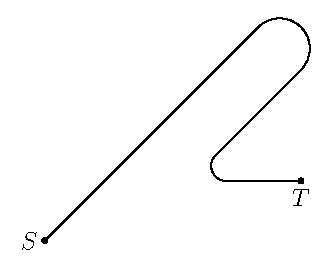
\includegraphics[viewport=234 339 377 452,clip]{nonhol.eps}\\
\caption{质点运动轨迹}\label{figure:coordinate}
\end{figure}

%\vspace*{5mm}
%\centerline{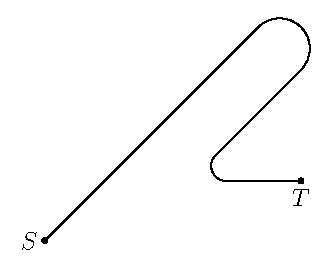
\includegraphics{nonhol.eps}}
%\vskip 2mm
%\centerline{{\footnotesize 图1 \quad 质点运动轨迹  }}
%\vskip 0.55\baselineskip

这个问题的多解性,是由于不同情形下质点受力情况不同。希望通过\eqref{eq:unit}来求得质点所受约束力进而求解质点的运动是不能实现的,实际上我们只能进行相反的求解,即根据已知的运动轨迹求出质点受力情况。
从图中也可以看出仅仅给定初始条件也是不够的,相同的初始条件,只要运动过程中受力情况不同,可以对应完全不同的运动。要完全求解质点的运动,必须给出质点在运动过程中的受力情况。实际上,从这个图也可以得到,只要有合适的控制作用质点可以运动到空间中任意位置,而这也正是非完整约束的特点。


这种观点其实可以推广到很多经典非完整系统中,例如斜面上冰刀运动问题,两轮小车问题,刚球在粗糙面纯滚动问题。满足它们各自非完整关系的运动有很多,不同模型给出的解实际上各自暗含了系统受力状况。不同的受力状况当然给出不同的方程和不同的解,即使它们都会满足非完整关系。从这个角度来说,无论是Chetaev模型还是Vacco动力学模型都与经典分析力学不矛盾,它们给出的解只要是满足所要求的非完整关系就是正确的,不同的只是它们各自暗含的控制力。Chetaev条件对应的正是一种控制力,即\eqref{eq:leom}的右端,在这种控制作用下可求得系统的运动。希望根据这个运动反求出所谓的非完整约束力当然只能再次得到这个控制力,因为它们本就是同一件事情。而Vacco模型则暗含的是另一种控制力情形,这种控制力使得系统修正后的作用量取驻值,运动的轨迹是测地轨道。在Vacco模型中更能体现非完整力学问题本质是控制问题的观点。显然我们也可以使用其他模型。只要我们给定或假设其他的控制力情形,那么得到的动力学方程当然不同于这两个模型,但只要不破坏预先要求的非完整关系它们仍然是正确的。


\section{结论}
\label{sec:conclusion}

在非完整系统的研究中,往往存在大量的争论,例如Lagrange原理和Hamilton原理的有效性,虚位移的定义,微分变分运算交换性等问题。人们通过对这些问题的讨论,加深了对非完整力学的认识,同时也得到了很多非完整系统的运动方程。但这些方程往往十分复杂而难于应用,而且根据不同的模型得到的方程还不协调。已有的矛盾和困惑促使我们必需关注非完整约束的物理实质。非完整约束是如何被抽象出来?非完整约束关系如何实现?本文正是从物理背景而不是数学分析出发来探讨这个问题。

作为例子,本文详细分析了冰刀运动解的合理性并讨论了冰刀运动的物理实现,解释了在冰刀运动中出现的所谓非完整力或跟随力的物理意义。

针对一般非完整系统,我们提出如下观点:

1.通常所说的非完整约束,应当称作非完整关系,这是系统在运动中必须满足的关系,可以作为描述运动的特征,或者是预先给定的系统运动的首次积分。非完整约束不具备完整约束在分析力学中的基础地位。其实,系统的首次积分或守恒量也可以看作是非完整约束,但除了一些简单的问题,仅靠这些首次积分并不能完全求解系统。例\ref{ex:unit}正是这样的例子,\eqref{eq:unit}可以认为是能量守恒量,但仅有这个守恒量不能确定问题的解。

2.不存在所谓的非完整力,即由于非完整约束导致的非完整约束力。令系统保持非完整关系的作用力是外界施加的控制力,这个力需要明确给定,或者是根据已知运动可确定出来。

3.非完整系统的求解需要明确给出系统的初始条件和系统的受力状况,只给出非完整关系的系统,其运动方程和解是不确定的。通过不同模型得到的解都是暗含了系统的受力状况。

4.非完整系统问题本质上是控制问题,即如何施加控制力来使系统进行目标运动。

或许从这样的角度可以更好的理解非完整系统:系统受到各种内力和外力的作用,作用的结果“碰巧”使得关系\eqref{eq:nhcon}成立。

\refrule

\begin{thebibliography}{999}

\bibitem{1} Hertz H 1894 Die Prizipien der Mechanik in neoen Zusammhage dargestellt (Leipzip: Barth)
\bibitem{2} Mei F X 1985 The Foundations of Mechanics of Nonholonomic System (Beijing: Beijing Institute of Technology Press) (in Chinese) [梅凤翔 1985 非完整系统力学基础 (北京: 北京工业学院出版社)]
\bibitem{3} Flannery M 2004 {\it Am. J. Phys.} {\bf 73} 265
\bibitem{4} Flannery M 2011 {\it Am. J. Phys.} {\bf 79} 932
\bibitem{5} Borisov A , Mamaev I 2002 {\it Regular and Chaotic Dynamics} {\bf 7} 43
\bibitem{6} Guo Z H , Gap P Y 1989 {\it Acta Mechanics Sinica} {\bf 5} 253
\bibitem{7} Bloch A 2003 Nonholonomic Mechanics and Control (Interdisciplinary Applied Mathematics Vol 24) (Berlin: Springer)
\bibitem{8} Luo S K , Zhang Y F 2008 Advances in the Study of Dynamics of Constrained Systems (Beijing: Science Press)
\bibitem{9} Greenwood D T 1977 Classical Dynamics (Englewood Cliffs: Prentice-Hall)
\bibitem{10} Neimark J , Fufaev N 1972 Dynamics of Nonholonomic Systems(Transactions of Mathematical Monographs Vol 33)(Providence: American Mathematical Society)
\end{thebibliography}

\newpage

\title{{\boldfont}%
Nonholonomic Mechanics and Control$^{\ast}$}

\author{Wang Dingwen$^{1)\dag}$ \quad  Gao Puyun$^{1)}$}

\email{wangdingwen0618@gmail.com  \quad tel: 15116442661}
\eaddress{1)}{
College of Aerospace Science and Engineering, National University of Defense Technology, Changsha $410072$,China}


\eabstract{The difficult of nonholonomic mechanics is due to the non-integrability of nonholonmic constraints. The origin of nonholonomic constraints is always ignored by researchers. We reveal the control essence of nonholonomic mechanics based on the physical meaning of nonholonomic constraints. From this point of view, the different models( such as Chetaev Model and Vacco Model) can be unified. We clarify that nonholonomic mechanics is still under the theory frame of analytical mechanics. It is the control forces implied by different models that distinguish them.
}
\ekeywords{Nonholonomic Mechanics, Control Theory, Chetaev Model, Vacco Model}


\epacs{45.05.+x,45.20.Jj,45.80.+r}


\newpage
\vspace*{5mm}
\centerline{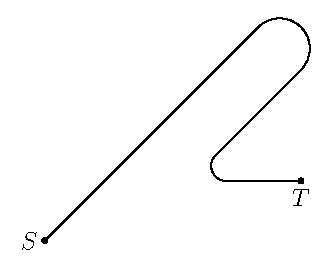
\includegraphics[viewport=234 339 377 452,clip]{nonhol}}
%\vspace*{6mm}
\vskip 2mm
\centerline{{\footnotesize 图1 \quad 质点运动轨迹}}
\vskip 0.55\baselineskip

\end{document}